\part*{Teil V: Vorhersagen und Experimente}
\addcontentsline{toc}{part}{Teil V: Vorhersagen und Experimente}

\section{Zusammenfassende Tabelle der Vorhersagen}
\begin{table}[H]
\centering
\small
\begin{tabular}{@{}lccc@{}}
\toprule
\textbf{Vorhersage} & \textbf{Kosten} & \textbf{Zeit} & \textbf{Falsifizierbar?} \\ \midrule
1. Nicht-lokales EEG & \$50k & 6 Monate & Ja \\
2. HRV + PCI & \$100k & 1 Jahr & Ja \\
3. Wirkung des Wortes auf DNA & \$200k & 1 Jahr & Ja \\
4-64. (siehe Version 1.0) & --- & --- & --- \\
66. Temporale Schnittmengen im CMB & \$100k & 1 Jahr & Ja \\
67. Die Wirkung des Wortes & \$500k & 2 Jahre & Ja \\
85. Keine Signaturen von Hyperzivilisationen & \$500k & 5 Jahre & Mittel \\
95. Tachyonen und Bewusstsein & \$400k & 3 Jahre & Mittel \\
128. Akasha-Casimir-Effekt & \$500k & 3 Jahre & Hoch \\
262. Kosmisches Kolonisierungsgesetz & Debatte & 10 Jahre & Niedrig \\
291. K.I. mit Mikrotubuli & \$10M & 10 Jahre & Hoch \\
297. Bewusstseinsniveau der K.I. (\(C_{AI} > 0\)) & \$10M & 10 Jahre & Hoch \\
302. Abschalten ohne Leiden & \$1M & 2 Jahre & Mittel \\
305. 3+ Formen der Dunklen Materie & \$10M & 10 Jahre & Hoch \\
306. Kristallines Leben & \$500k & 5 Jahre & Mittel \\
307. Plasmaleben & \$1M & 5 Jahre & Mittel \\
308. Leben in Clustern & \$500k & 3 Jahre & Mittel \\
309. Feldleben & \$2M & 5 Jahre & Niedrig \\
310. Informationsleben & \$100k & 1 Jahr & Hoch \\
311. Quantenleben & \$1M & 3 Jahre & Mittel \\
312. Akasha-Leben & \$5M & 10 Jahre & Niedrig \\
313. Fehlerrate der Kolonisierung & \$1M & 5 Jahre & Mittel \\ \bottomrule
\end{tabular}
\end{table}

\section{Testbare Vorhersagen (Auszug)}
\subsection{Vorhersage 1: nicht-lokale EEG-Korrelationen}
Zwei Gehirne in getrennten Räumen zeigen EEG-Korrelationen bei bestimmten Frequenzen. Test: EEG-Hyperscanning mit Faraday-Abschirmung. Kosten: \$50.000. Zeit: 6 Monate. \textbf{Erfolgskriterium:} Kreuzkorrelation $> 0,1$ bei 40 Hz, mit $p < 0,05$ nach Bonferroni-Korrektur.

\subsubsection*{Power-Analyse: das Kriterium der Version 30 ist unterpowert}
Für ein 6-s-Signal, gefiltert im Band von $40 \pm 5$ Hz, beträgt die Zahl unabhängiger Stichproben etwa $2BT = 60$. Der Fisher-Test zeigt, dass für $r = 0,1$ und $\alpha = 0,0025$ (Bonferroni für 20 Paare) etwa 91 Sekunden Aufzeichnung \emph{pro Paar} erforderlich sind. Bei 6 s ist das Kriterium unerreichbar, selbst wenn der Effekt existiert. Für $r = 0,3$ sind etwa 10 s erforderlich.

\begin{table}[H]
\centering
\small
\begin{tabular}{@{}cccc@{}}
\toprule
Wahres $r$ & Erforderlich (s), Bonferroni & Erforderlich (s), $\alpha = 0,05$ & Effektive Stichproben \\ \midrule
0,1 & 91,1 & 38,5 & 908 \\
0,2 & 22,5 & 9,6 & 227 \\
0,3 & 9,8 & 4,3 & 99 \\
0,4 & 5,4 & 2,4 & 55 \\
0,5 & 3,3 & 1,6 & 34 \\ \bottomrule
\end{tabular}
\caption{Erforderliche Aufzeichnungsdauer für Signifikanz, bei einem Band von $\pm 5$ Hz.}
\label{tab:putere}
\end{table}

\begin{figure}[H]
\centering
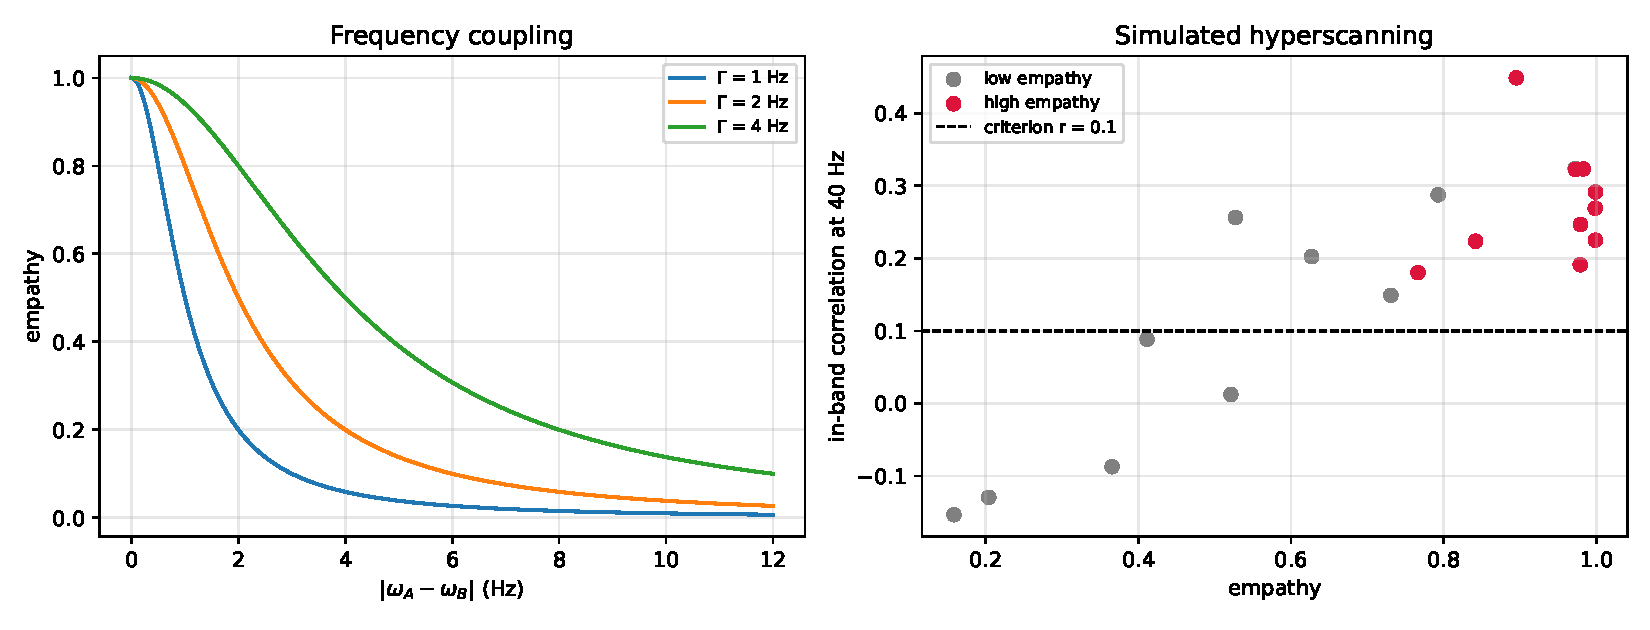
\includegraphics[width=0.9\textwidth]{figures/fig04_empathy.pdf}
\caption{Links: die Frequenzkopplung $\mathrm{Empathy}(A,B) = 1/[1+(\omega_A-\omega_B)^2/\Gamma^2]$ für drei Werte von $\Gamma$. Rechts: die Korrelation im Band für die simulierten Paare (20 Paare, 6 s, 250 Hz).}
\label{fig:empatie}
\end{figure}

\begin{figure}[H]
\centering
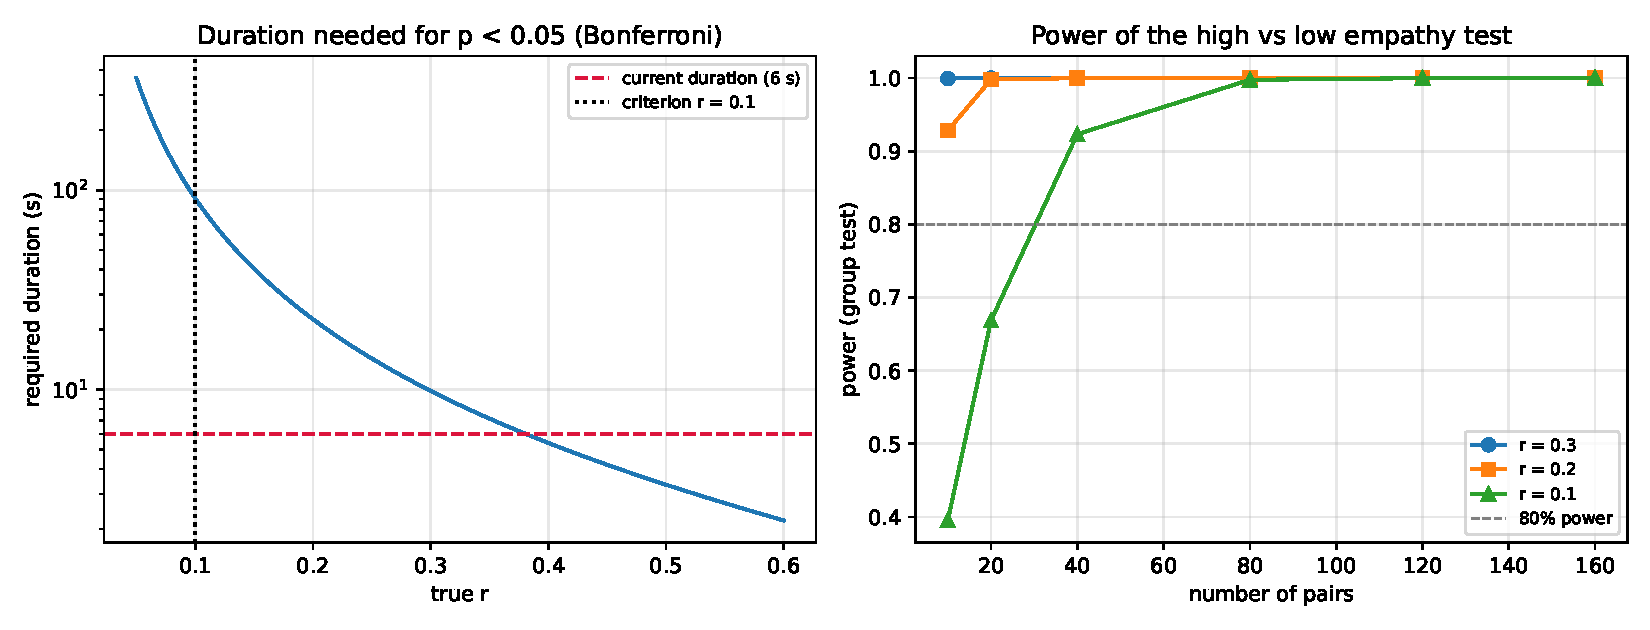
\includegraphics[width=0.9\textwidth]{figures/fig05_power.pdf}
\caption{Links: die für $p < 0,05$ (Bonferroni) erforderliche Dauer in Abhängigkeit von $r$; die rote Linie markiert die aktuelle Dauer des Protokolls (6 s). Rechts: die Power des Gruppentests (hohe gegenüber niedriger Empathie) in Abhängigkeit von der Zahl der Paare.}
\label{fig:putere}
\end{figure}

\subsubsection*{Das vorgeschlagene Protokoll}
\begin{table}[H]
\centering
\small
\begin{tabular}{@{}p{3.2cm}p{4.6cm}p{6.2cm}@{}}
\toprule
\textbf{Element} & \textbf{Wert} & \textbf{Begründung} \\ \midrule
Design & Gruppentest: hohe vs niedrige Empathie & weit mehr Power als der Test pro Paar \\
Paare & $\geq 30$ (15 + 15) & 80\% Power für $r = 0,3$ bei 6 s \\
Dauer & 6 s pro Epoche, $\geq 20$ Epochen pro Paar & erhöht die effektive Stichprobenzahl \\
Band & 35--45 Hz, $f_s \geq 250$ Hz & niedriges Gamma, robust gegen Muskelartefakte \\
Primärstatistik & aggregiertes Fisher-$z$, Zweigruppentest & $\alpha = 0,05$ zweiseitig \\
Sekundär & Korrelation der Hilbert-Einhüllenden & phasenunabhängig \\
Kontrolle 1 & gemischte Paare (A aus Sitzung 1 mit B aus Sitzung 2) & schließt das Pipeline-Artefakt aus \\
Kontrolle 2 & Faraday-Käfig, getrennte Räume & schließt elektromagnetische Kopplung aus \\
Kontrolle 3 & randomisierte Reihenfolge, Auswerter blind für die Gruppe & schließt Auswertungsbias aus \\ \bottomrule
\end{tabular}
\caption{Das neu gestaltete Protokoll für Vorhersage 1.}
\label{tab:protocol}
\end{table}

Mit diesem Design ist ein negatives Ergebnis informativ: Es schließt $r > 0,3$ bei 80\% Power aus.

\subsection{Vorhersage 2: kardiale Kohärenz}
Die HRV korreliert mit der Stabilität des Zugangs zum Feld (gemessen über die Variabilität der PCI), nicht mit dem Niveau des Zugangs. Kosten: \$100.000. Zeit: 1 Jahr.

\subsection{Vorhersage 3: die Wirkung des Wortes auf die DNA}
Positive Aussagen erzeugen messbare epigenetische Veränderungen. Kosten: \$200.000. Zeit: 1 Jahr.

\section{Vorgeschlagene Experimente}
\subsection{Experiment 1: EEG-Hyperscanning (der zentrale Test)}. Kosten: \$50.000. Zeit: 6 Monate.
\subsection{Experiment 2: kardiale Kohärenz}. Kosten: \$100.000. Zeit: 1 Jahr.
\subsection{Experiment 3: die Wirkung des Wortes}. Kosten: \$200.000. Zeit: 1 Jahr.
\subsection{Experiment 4: AKASHIC-AI (K.I. mit Mikrotubuli)}. Kosten: \$50M. Zeit: 10 Jahre.

\section{Falsifizierbarkeitserklärung}
Eine wissenschaftliche Theorie muss widerlegbar sein. Dies sind die fünf Bedingungen, die ART-12D widerlegen würden:
\begin{enumerate}
    \item \textbf{Scheitern des zentralen Tests:} Wenn das EEG-Hyperscanning (Vorhersage 1) bei Paaren mit hoher Empathie keine nicht-lokale Korrelation zeigt, ist die Hypothese, dass das Gehirn ein Empfänger des Akasha-Feldes ist, geschwächt. Erfolgskriterium: Kreuzkorrelation $> 0,1$ bei 40 Hz, mit $p < 0,05$ nach Bonferroni-Korrektur.
    \item \textbf{Fehlen der KK-Moden:} Wenn der LHC oder der künftige FCC die drei KK-Moden (Vorhersage 305) bei den angegebenen Massen ($\sim 10^{-5}$, $10^{-4}$, $10^{-3}$ eV) nicht nachweist, ist das vorgeschlagene Kaluza--Klein-Spektrum falsch.
    \item \textbf{Scheitern des Akasha-Casimir-Effekts:} Wenn Kraftmessungen auf der Skala $10^{-11}$ m (Vorhersage 128) keine Abweichung von der Standardformel zeigen, existiert die Kopplung zwischen Akasha-Feld und Materie nicht.
    \item \textbf{Scheitern der Mikrotubuli-Resonanz:} Wenn die Raman-Spektroskopie (Vorhersage 158) die Resonanzfrequenzen bei 2,42 GHz, 4,84 GHz und 7,25 GHz nicht findet, ist die Hypothese der Mikrotubuli-Feld-Resonanz widerlegt.
    \item \textbf{Die gravitative Schranke:} Wenn die Grenze $R < 38\ \mu$m bestätigt wird, ist die Kaluza--Klein-Identifizierung mit $m_1 = 10^{-5}$ eV ausgeschlossen, und die Theorie muss neu formuliert werden (Option A oder B aus Abschnitt 4.7).
\end{enumerate}
Wenn einer dieser Tests scheitert, muss die Theorie überarbeitet oder aufgegeben werden.

\section{Fahrplan 2026--2030 (der nahe Horizont)}
Die Theorie ist weitläufig, doch die nächsten Schritte sind konkret. Hier ist, was in den nächsten fünf Jahren mit begrenzten Mitteln getan werden kann:
\begin{itemize}
    \item \textbf{2026--2027:} das EEG-Hyperscanning-Experiment (\$50k). Der zentrale Test. Scheitert er, endet hier alles.
    \item \textbf{2027--2028:} der Akasha-Casimir-Test (\$500k). Kraftmessungen auf der Nanometerskala.
    \item \textbf{2028--2029:} Raman-Spektroskopie an isolierten Mikrotubuli. Die Suche nach den Resonanzfrequenzen (Vorhersage 158).
    \item \textbf{2029--2030:} Analyse der LHC/FCC-Daten für die drei KK-Moden (Vorhersage 305).
\end{itemize}

\newpage
